\newpage
\subsection{Планирование сырья}
\label{bp:RawMaterialPlanning}

\textbf{Планирование бумаги и картона}

Макулатурное сырье поступает с ООО ''ПЗБМ''. Целлюлозное сырье поступает от сторонних производителей АО ''АЦБК'' и  АO ''CЛПК''.

Планирование основного сырья (бумага и картон) происходит один раз месяц.
Планированием бумаги и картона и крахмала занимается начальник отдела планирования. 
Отдел планирования ведет контроль за уже размещенными заявками (рис. \ref{pic:VII 6}) в MS Excel.

Поставщики требуют размещения заявок на производство до 20 числа каждого месяца. На ПРЕДПРИЯТИИ принято иметь страховой запас как минимум на 1,5 месяца. Потребность в сырье определяется на основании статических данных за расчетный период. 

Заявки оформляются в MS Word. 

Все заявки согласовываются с директором ПРЕДПРИЯТИЯ.

Заявка на АО ''АЦБК'' размещается (отправляется по почте) на месяц без указаний весовых характеристик и форматов (рис. \ref{pic:VII 7}).  Еженедельно с поставщиком утверждается граммаж (вес м2), формат и количество рулонов.
Заявка на АO ''CЛПК'' размещается на месяц с указанием граммажа (вес м2)  и форматов (рис. \ref{pic:VII 8}). Еженедельно согласовывается и корректируется с поставщиком план отгрузок по размещенной заявке.

Начальник отдела планирования производит расчет месячной потребности в сырье, производимом ООО ''ПЗБМ''. Для этого начальник отдела планирование собирает информацию из разных отчетов в системе 1С: УПП.
Расчет потребности в сырье, производимом ООО ''ПЗБМ'', производится в MS Excel.
Расчет выполняется на основе текущих остатков по сырью из отчета из 1С: УПП по рулонам (рис. \ref{pic:VII 9}).

На ПРЕДПРИЯТИИ используются утвержденные композиции (рис. \ref{pic:VII 3}). Фантомы сырьевых номенклатур представлены на рис. \ref{pic:VII 2}.

Сформированная заявка на поставку ролевой продукции ООО ''ПЗБМ'' согласовывается с директором ПРЕДПРИЯТИЯ.


 \clearpage
 
\begin{figure}
\begin{center}
 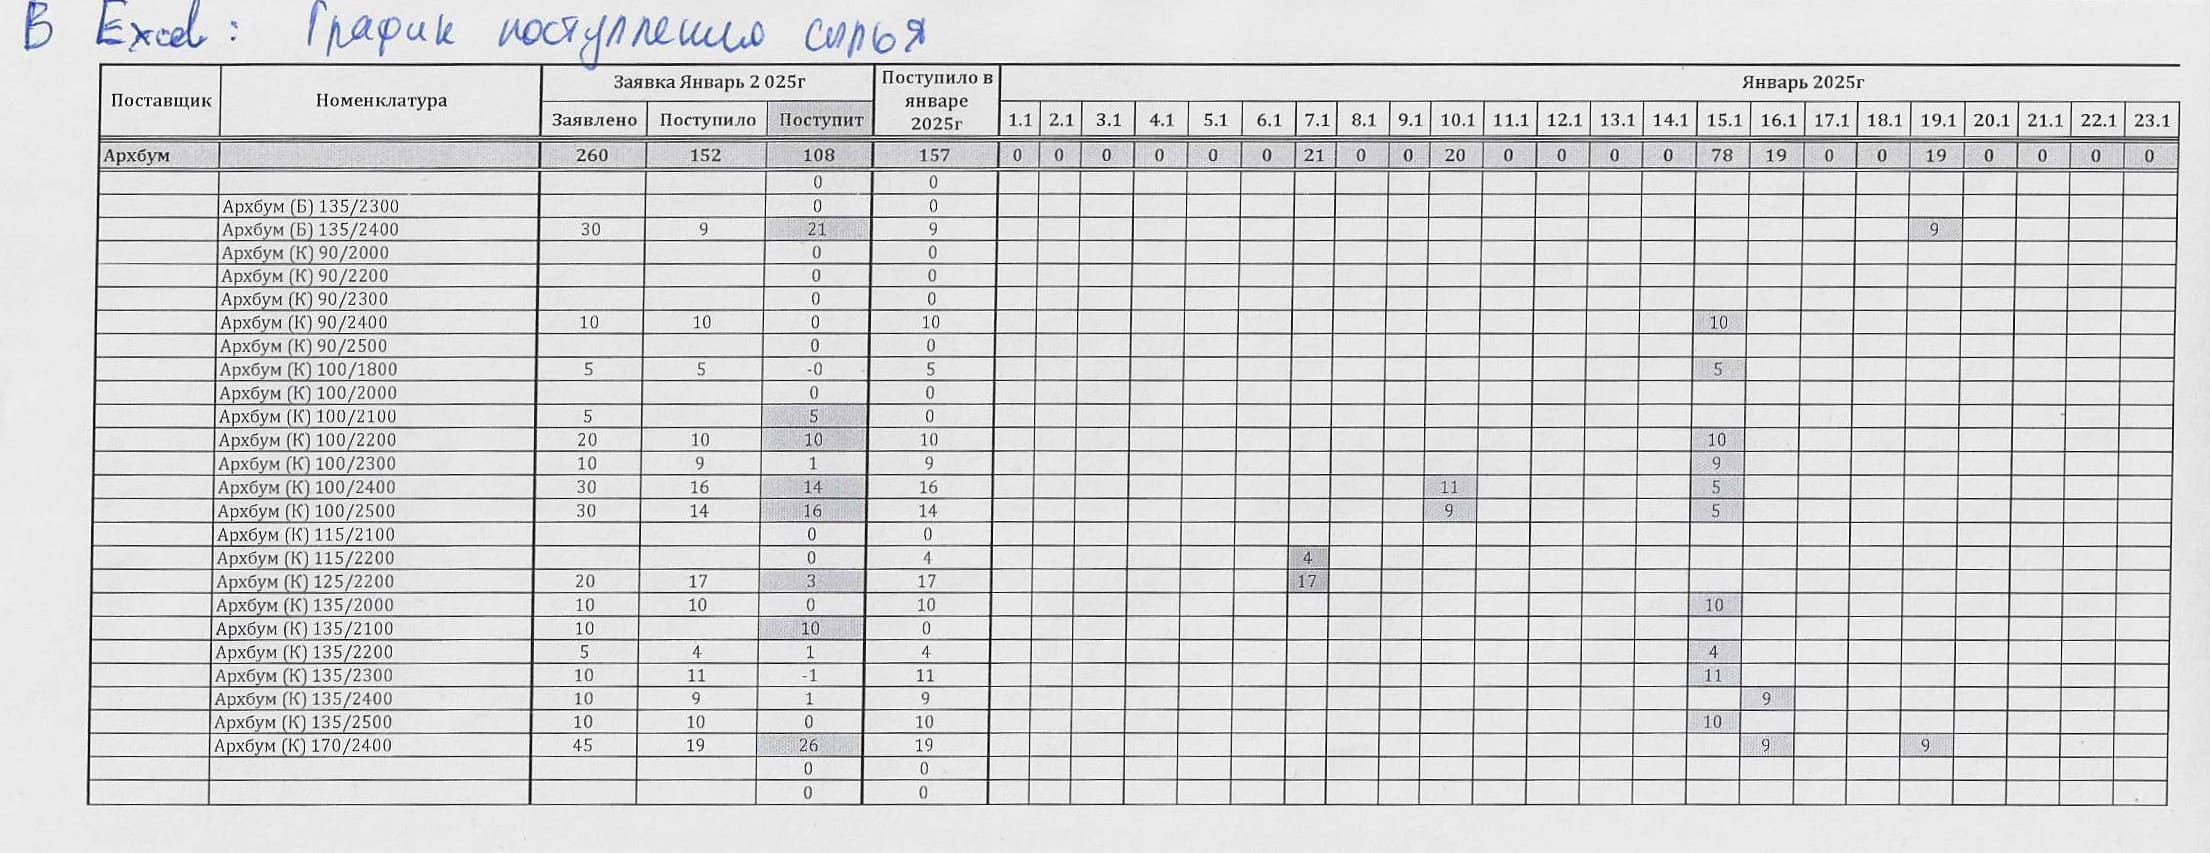
\includegraphics[height=0.35\textheight, angle=90, keepaspectratio]{Pics/VII 6.jpg}
\end{center}
 \caption{График поставок ролевого сырья от поставщика АО ''АЦБК''}
 \label{pic:VII 6}
\end{figure}


\begin{figure}
\begin{center}
 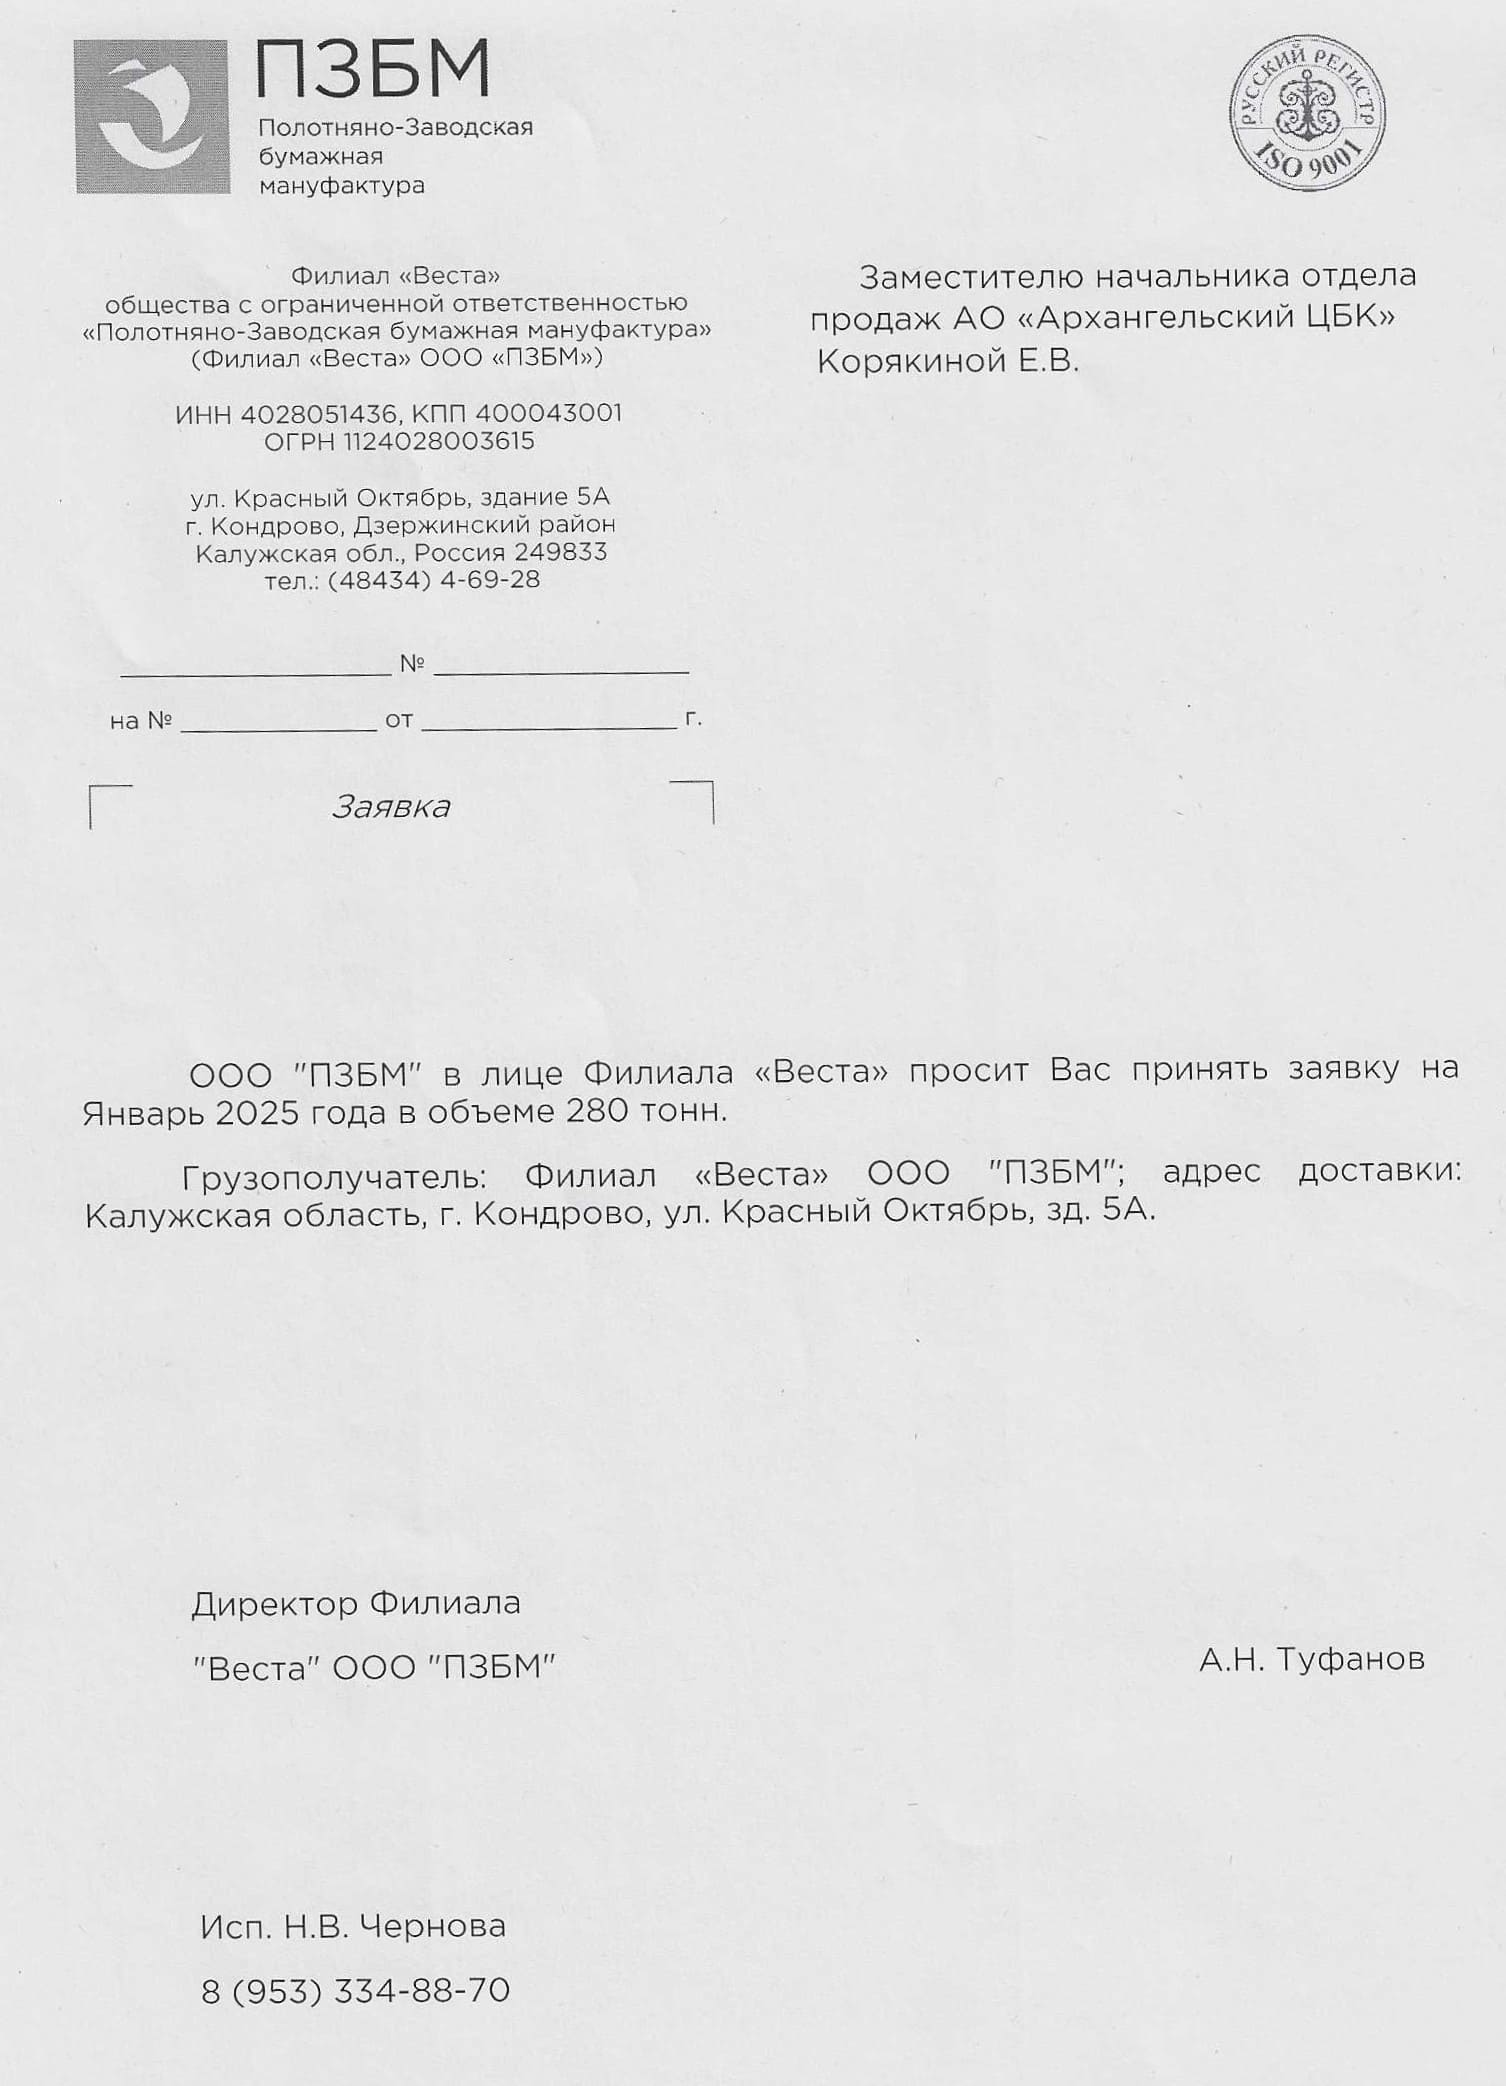
\includegraphics[height=0.6\textheight, keepaspectratio]{Pics/VII 7.jpg}
\end{center}
 \caption{Заявка на поставку ролевого сырья АО ''АЦБК''}
 \label{pic:VII 7}
\end{figure}

\begin{figure}
\begin{center}
 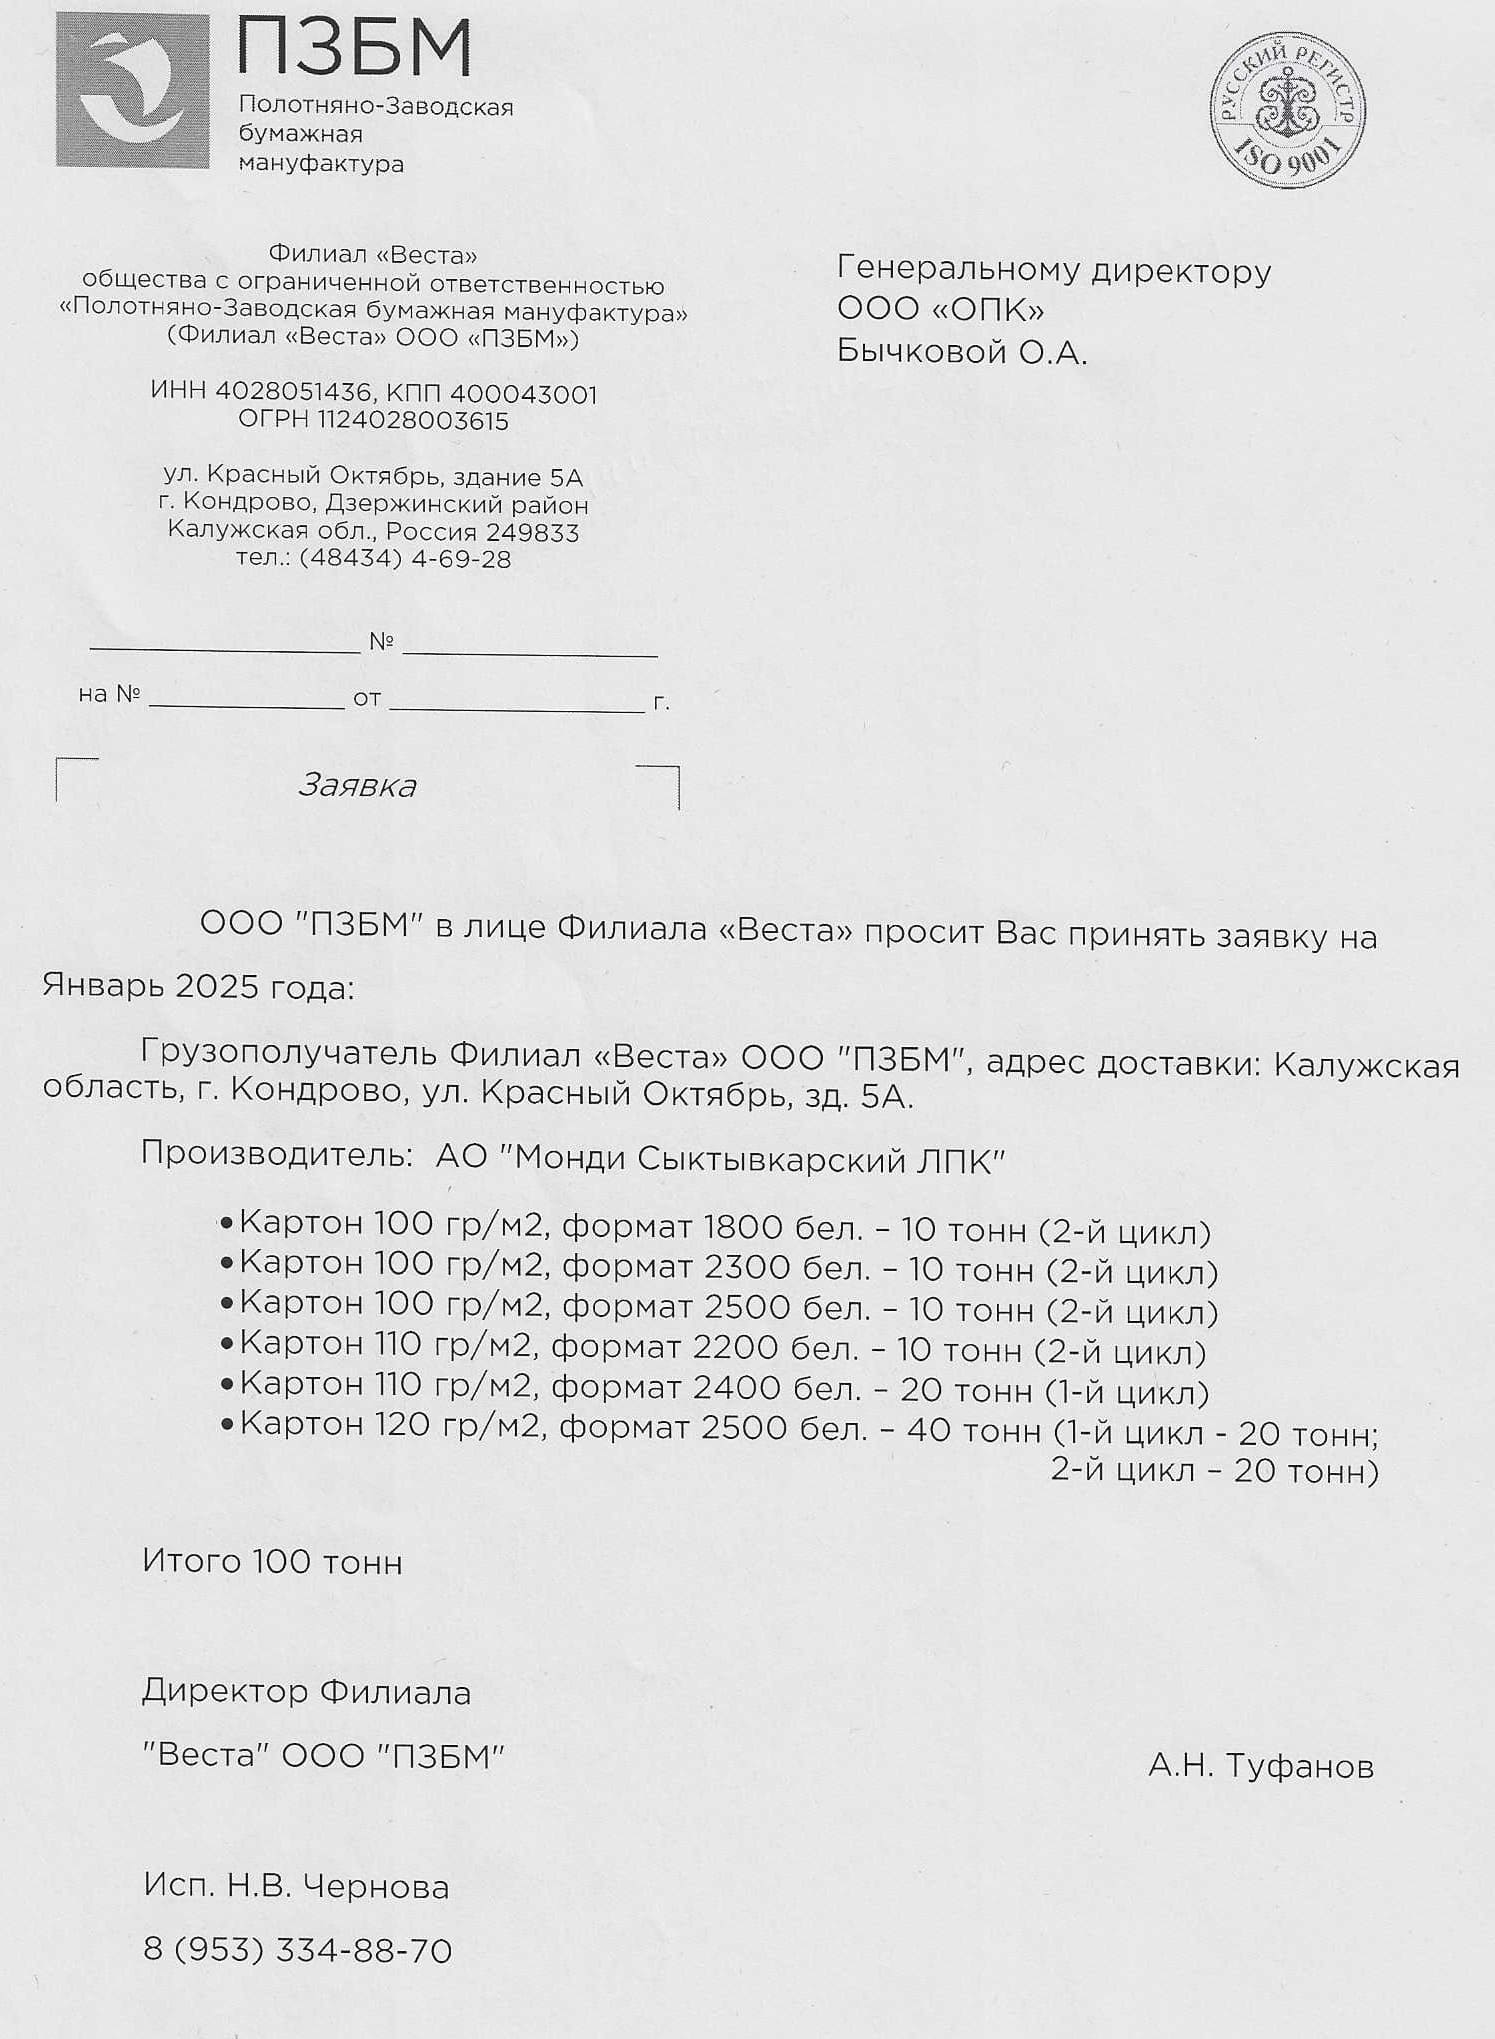
\includegraphics[height=0.6\textheight, keepaspectratio]{Pics/VII 8.jpg}
\end{center}
 \caption{Заявка на поставку ролевого сырья Монди}
 \label{pic:VII 8}
\end{figure}

\begin{figure}
\begin{center}
 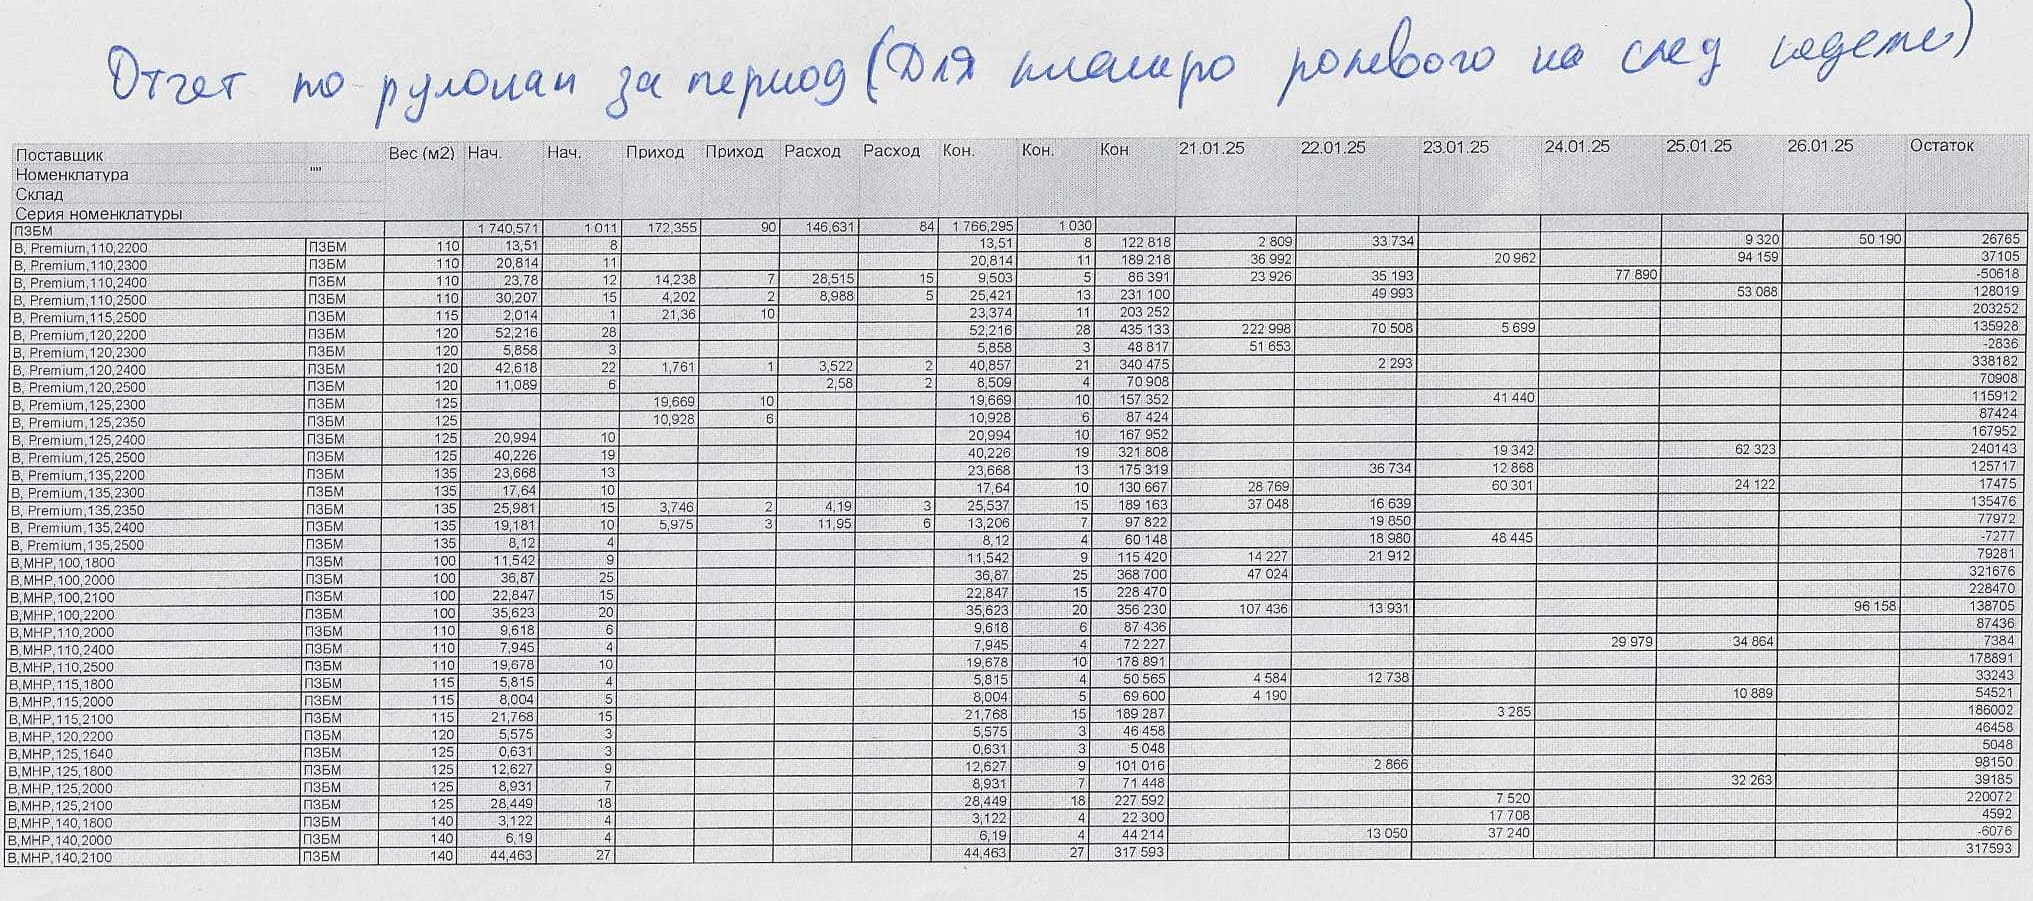
\includegraphics[height=0.25\textheight, keepaspectratio]{Pics/VII 9.jpg}
\end{center}
 \caption{Отчет по рулонам за определенный период в 1С: УПП}
 \label{pic:VII 9}
\end{figure}

\begin{figure}
\begin{center}
 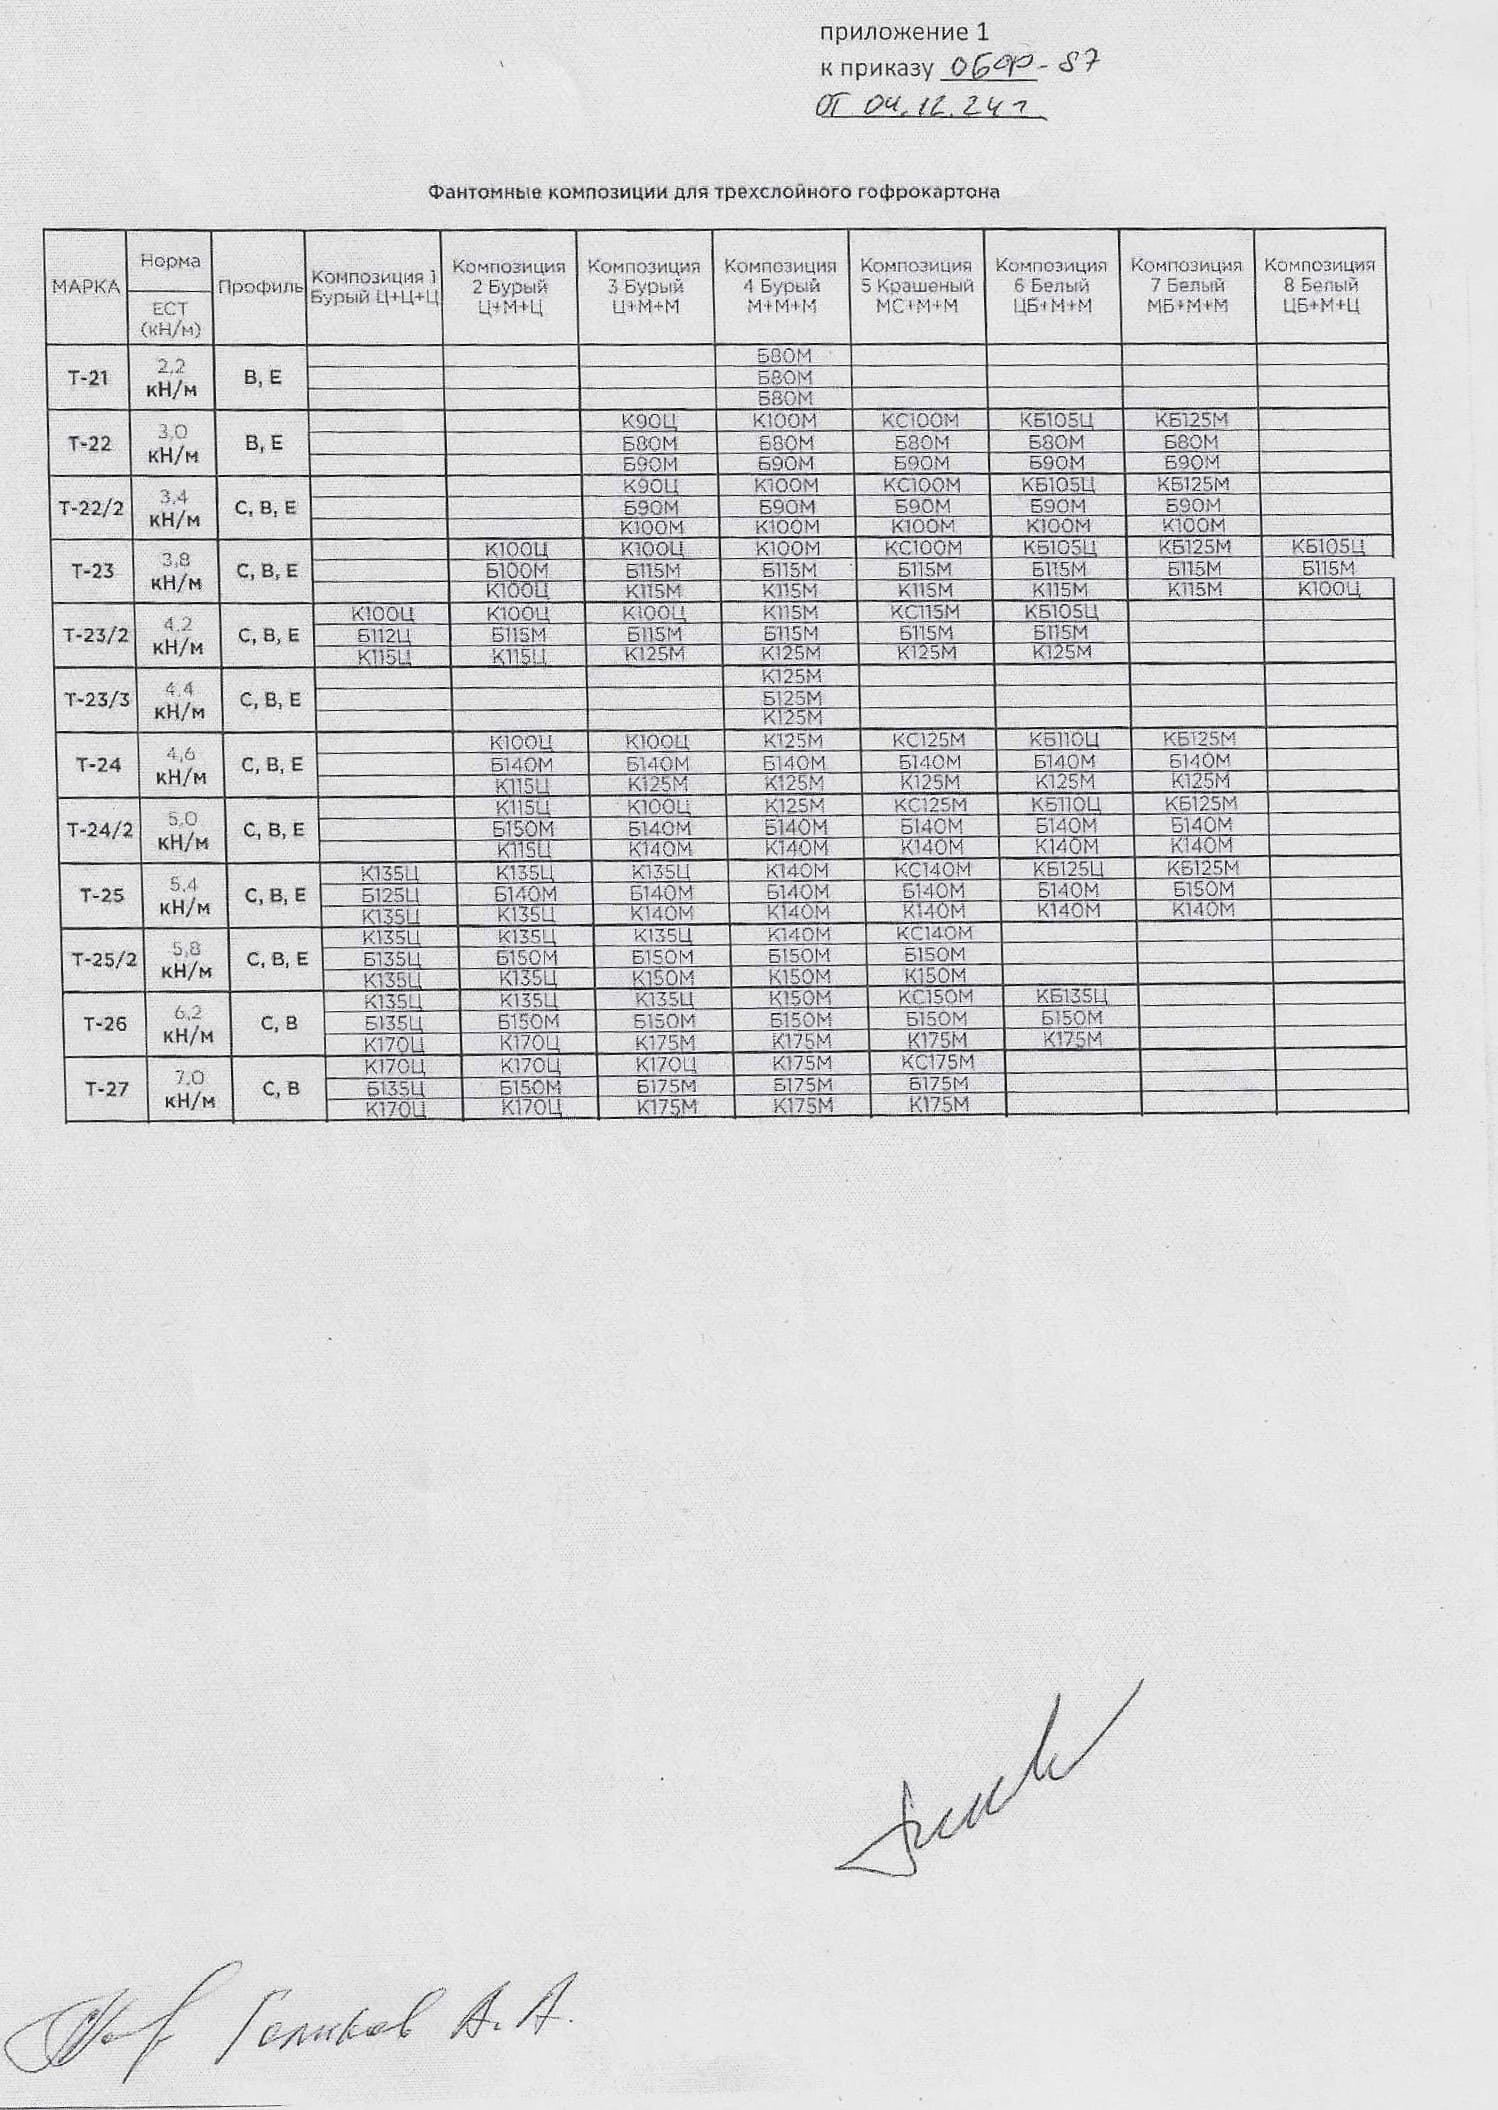
\includegraphics[height=0.8\textheight, keepaspectratio]{Pics/VII 3.jpg}
\end{center}
 \caption{Утвержденные фантомные композиции}
 \label{pic:VII 3}
\end{figure}

\begin{figure}
\begin{center}
 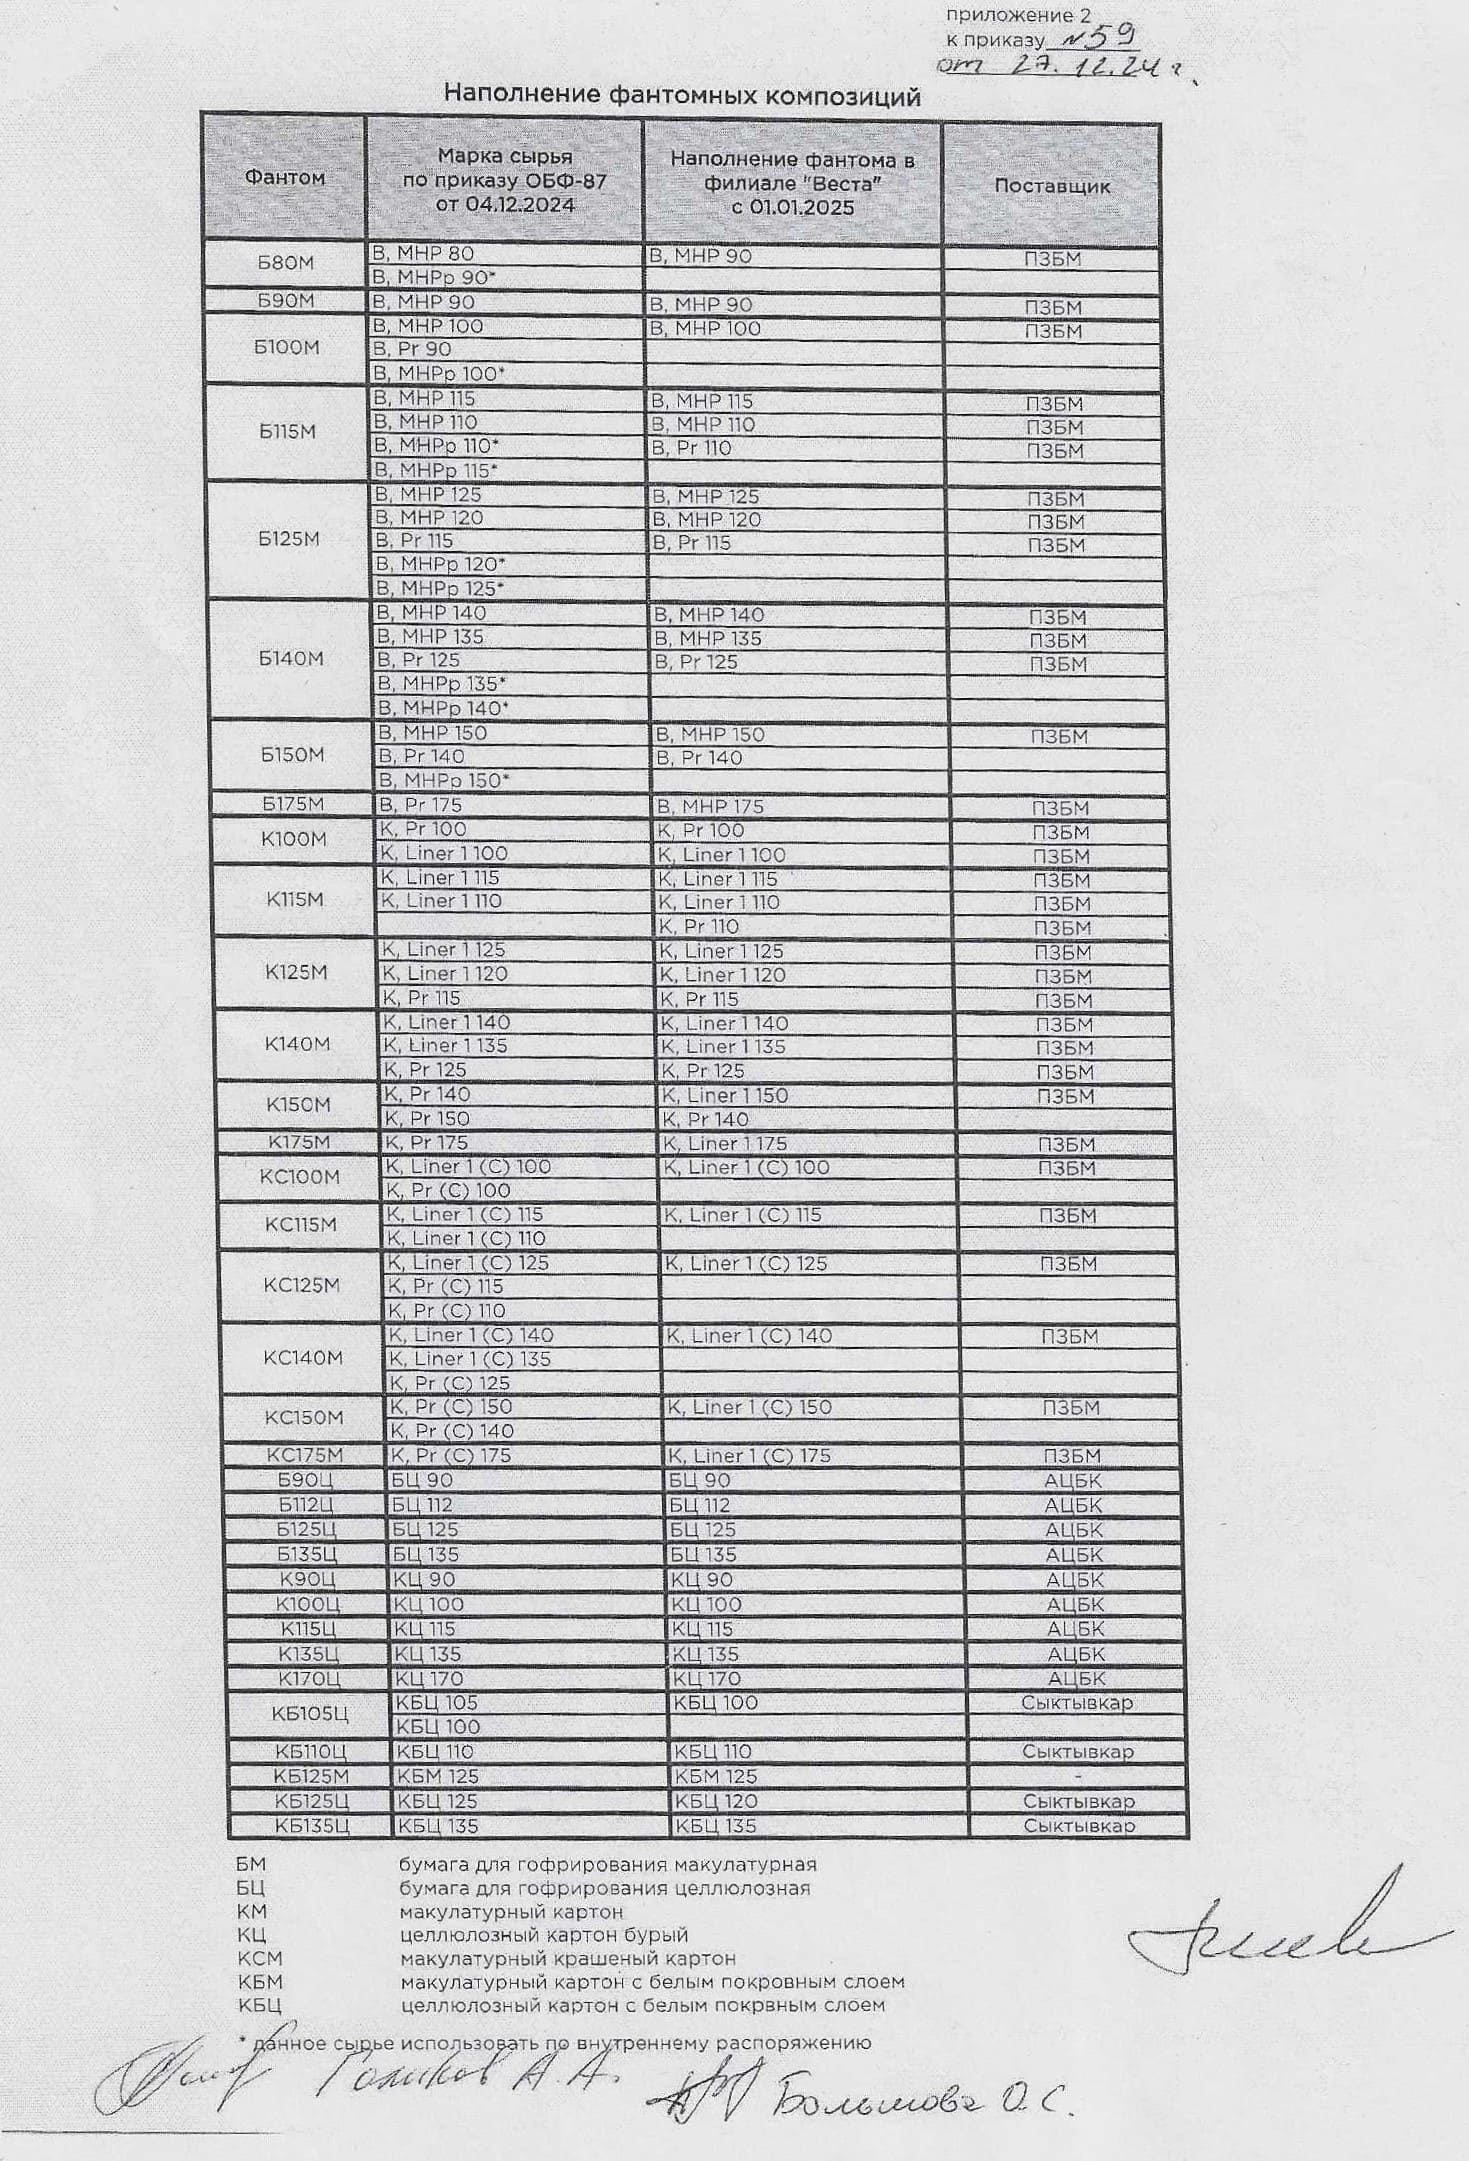
\includegraphics[height=0.8\textheight, keepaspectratio]{Pics/VII 2.jpg}
\end{center}
 \caption{Утвержденное наполнение фантомных композиций}
 \label{pic:VII 2}
\end{figure}

\clearpage

















% Планирование основного сырья (бумага и картон) выполняет генеральный директор.
% На гофроагрегате при использовании сырья разработан нормативный документ по возможным заменам сырья. 
% Планирование сырья выполняется в конце месяца на будущий месяц.
% Генеральный директор из системы СБИС формирует отчет по остаткам картона (рис. \ref{pic:d31}). На основании отчета \ref{pic:d31} генеральный директор руками создает отчет по потребностям в сырье в таблице MS Excel (рис. \ref{pic:d30}).
% Генеральный директор на основании созданной формы выполняет расчет в потребностях и формирует заявки на закупку сырья поставщикам.
% Заявки в виде писем по емайл рассылаются поставщикам. В случае отказа поставщика генеральный директор выбирает другого альтернативного по данному виду сырья. Генеральный директор оговаривает цену с поставщиками. Заявка поставщику отсылается по электронной почте (рис. \ref{pic:d32}).






















% \textbf{Планирование закупки заготовок}

% На производстве выделены популярные позиции заготовок, по которым имеется складской запас. 


% По таким изделиям МСЗ контролируют объем неснижаемого запаса вручную и при необходимости создают заказы покупателя на контрагента ООО ''Рускартон'' (на склад). 
% Остальные заготовки поступают сразу в производство под конкретный производственный заказ.
% МСЗ на основании заказа покупателя создает заказ на бронь по складским свободным остаткам. Остатки МСЗ может узнать по отчету в 1С:УНФ «Остатки ГП». В момент отгрузки менеджер снимает с резерва свободные остатки в разрезе заказа покупателя.

% Планированием закупки заготовок занимается инженер по планированию.
% Заказ от менеджера поступает в системе 1С:УНФ инженеру по планированию, который на основании плана производства в таблице MS Excel (рис. ??) создает в системе 1С:УНФ документ ''Заявка на продажу'' (рис. \ref{pic:d17}). 

% % \todo{перечитать с планированием}

% При создании заказа менеджеры стараются создавать заказ на производство кратно поддону. 
% Инженер по планированию ставит в системе 1С:УНФ у документа ''Заказ на производство'' статус «В работе» и заказывает заготовки у поставщиков согласно заказам на производство. Объем заказа заготовок в точности совпадает с объемом заказа на производство.
% На основании формы \ref{pic:d15} инженер по планированию формирует заявку на производство (заготовки) и заявку на ресурсе поставщика.

\textbf{Планирование вспомогательных материалов}



На ПРЕДПРИЯТИИ существует отлаженная система поставщиков по всем видам вспомогательных материалов. Каждое подразделение в зоне ответственности за основное производство сам занимается контролем/планированием/закупкой/заменой/ремонтом и т.д. с соответствующим поиском поставщиков/подрядчиков. Все новые договора с поставщиками, подрядчиками, контрагентами и т.д. контролируются через ''ПЕРВАЯ ФОРМА''. По каждому направлению утверждена группа, которая имеет право согласовывать закупки. 









% Планированием и закупкой вспомогательных материалов занимается отдел снабжения.

% Каждый день техник по учету определяет остатки по крахмалу и другим материалам (Пленка, скотч и др.) в производстве и сообщает по телефону в отдел снабжения остатки на складе. 25 числа каждого месяца менеджер по снабжению заказывает поставки крахмала на следующий месяц. Объемы заказа определяются коллективно с техником по учету. Менеджер отдела снабжения обзванивает поставщиков по ценам, формирует заявку в свободной форме. Поставки крахмала выполняются 2-3 раза в месяц.

% В системе СБИС хранятся текущие остатки на складах, но отдел снабжения не использует систему СБИС.


% По закупке других материалов (СИЗ, спецодежда, комплектующие и запчасти) отдел снабжения собирает заявки от подразделений, обрабатывает их, ищет поставщиков и производит закупку.


% Поддоны.

% Начальник склада каждый вечер определяет потребность по поддонам и сообщает по телефону в отдел снабжения, где менеджеры отдела снабжения фиксирует вручную объемы потребности.
% Коммерческий отдел и отдел снабжения совместно определяют потребность в поддонах исходя из плана производства и текущих остатков на складах и заказывают поддоны у производителей.
% Менеджеры отдела снабжения создают заявку на закупку поддонов и спецподдонов. Все поддоны невозвратные.
% Поддоны принимаются на складе. Учет поступления фиксируется в системе СБИС.


\textbf{Планирование краски }

%\todo{ПИСАТЬ}

На ПРЕДПРИЯТИИ установлена станция краскосмешения. Расчет потребности в краске отсутствует. Заказывают пигменты и сами готовят краску по рецептам. Контроль за остатками и заказом пигментов осуществляет технологический отдел.  





% Краску заказывает техник УВФ. Остатки основы и пигментов краски техник определяет визуально и по опыту заказывает необходимый объем напрямую у поставщика.



%Оснастку тоже.

% Закупками краски занимается инженер по планированию. Краска в цеху списывается ежедневно. Инженер по планированию ориентируясь на недельный план в таблице MS Excel, составляет потребность в краске на неделю и сравнивает с остатками в 1С (рис. \ref{pic:a80}). При наличии нужного пантона менее 20 кг (1 ведра), заказывается еще 20 кг.

% \begin{figure}
% \begin{center}
%   \includegraphics[height=0.6\textheight, keepaspectratio]{Pics/a80.jpg}
% \end{center}
%   \caption{Остатки по краске}
%   \label{pic:a80}
% \end{figure}
% \clearpage

% \textbf{Планирование вспомогательных материалов }

% Вспомогательные материалы закупает инженер по планированию. Списание на производстве происходит в конце месяца. По просьбе инженера по планированию кладовщик может пересчитать и предоставить остатки на бумаге (\ref{pic:a57}). Ориентируясь на них инженер по планированию закупает необходимые материалы. Клей закупает на месяц 240 кг (1 бочка).

% Мастер производства заказывает поддоны  по телефону, контролирует остатки  и заказывает недостающее количество. Перемещение поддонов выполняет  бухгалтер по накладной (\ref{pic:a31}). Поддоны от поставщиков (приходит заготовка) сразу увозят на другую площадку для сортировки. 

% \begin{figure}
% \begin{center}
%   \includegraphics[height=0.6\textheight, keepaspectratio]{Pics/d31.jpg}
% \end{center}
%   \caption{Отчет по остаткам картона}
%   \label{pic:d31}
% \end{figure}
% \clearpage

% \begin{figure}
% \begin{center}
%   \includegraphics[height=0.6\textheight, keepaspectratio]{Pics/d30.jpg}
% \end{center}
%   \caption{Форма для планирования потребности в бумагие и картоне}
%   \label{pic:d30}
% \end{figure}
% \clearpage

% \begin{figure}
% \begin{center}
%   \includegraphics[height=0.6\textheight, keepaspectratio]{Pics/d32.jpg}
% \end{center}
%   \caption{Форма заявки поставщику}
%   \label{pic:d32}
% \end{figure}
% \clearpage


% %
% \clearpage
% \ifx \notincludehead\undefined
\normalsize
\end{document}
\fi